\documentclass[11pt,a5paper]{article}

\usepackage[T1]{fontenc}
\usepackage[utf8]{inputenc}
\usepackage{lmodern, microtype}
\usepackage[estonian]{babel}
\usepackage[per=fraction, expproduct=cdot, decimalsymbol=comma, inter-unit-product=\cdot]{siunitx}
\usepackage{graphicx}
\usepackage{wrapfig}
\usepackage{tikz}
\usepackage[european]{circuitikz}
\tikzset{component/.style={draw,thick,circle,fill=white,minimum size=0.75cm,inner sep=0pt}}
\usepackage{amsmath,amssymb}
\usepackage{amsfonts}
\usepackage{hyperref}
\usepackage{csquotes}
\usepackage{caption}
\usepackage{enumitem}
\topmargin=-3.0cm \textheight=19cm \textwidth=12.9cm
\oddsidemargin=-1.5cm  \evensidemargin=-1.5cm
\setlength{\parindent}{0pt} \setlength{\parskip}{6pt} \sloppy
\sloppy \relpenalty=10000 \binoppenalty=10000
\pagestyle{empty}

\newcommand{\numb}[1]{\vspace{5pt}\textbf{\large #1}}
\newcommand{\nimi}[1]{(\textsl{\small #1})}
\newcommand{\punktid}[1]{(\emph{#1~p.})}
\newcounter{ylesanne}
\newcommand{\yl}[1]{\addtocounter{ylesanne}{1}\numb{\theylesanne.} \nimi{#1} \newblock{}}
% \newcommand{\autor}[1]{}
\newcommand{\autor}[1]{\emph{ Autor: #1}} %Temporarily surpressed



\begin{document}
\begin{center}
  \textbf{\Large Eesti koolinoorte 68. füüsikaolümpiaad} \par
  \emph{10. aprill 2021. a. Lõppvoor \\Gümnaasiumi ülesannete lahendused (10.--12. klass)}
\end{center}

\yl{LUMEPALL}
\punktid{6} \autor{Oleg Košik}
Lumepall peab läbima kiirendusega $g$ vertikaalse teepikkuse $H-h$, seega saame võrduse
$$H-h=\frac{gt^2}{2},$$ kus $t$ on lumepalli lennuaeg. Olgu $w$ lumepalli algkiirus, siis tema horisontaalsuunaline kiirus läheneva Richardi suhtes on $v+w$. Peab kehtima võrdus $$(v+w)t=l.$$ Avaldades esimesest võrdusest $t$ ja teisest $w$ leiame
$$w=l\sqrt{\frac{g}{2(H-h)}}-v\approx \SI{4,7}{m/s}.$$

\yl{PUDEL}
\punktid{6} \autor{Jarl Patrick Paide}
Toa jahedam õhk jahutab pudelit võimsusega $P$ saades pudelilt aja $t$ jooksul energia $\Delta Q = Pt$. Pudeli temperatuur muutub selle aja jooksul $\Delta T = \Delta Q/c$ võrra. Ideaalse gaasi olekuvõrrandist $PV=nRT$ saame temperatuuri muutusest rõhu muutuse $\Delta p = \frac{R \Delta T}{V_m} $. Pannes seosed kokku saame, et $P = \frac{\Delta p c V_m }{Rt}$

\yl{LÄÄTS JA EKRAAN}
\punktid{8} \autor{Oleg Košik}\par
\begin{figure}[!h]
  \centering
  \begin{minipage}[c]{0.39\textwidth}
    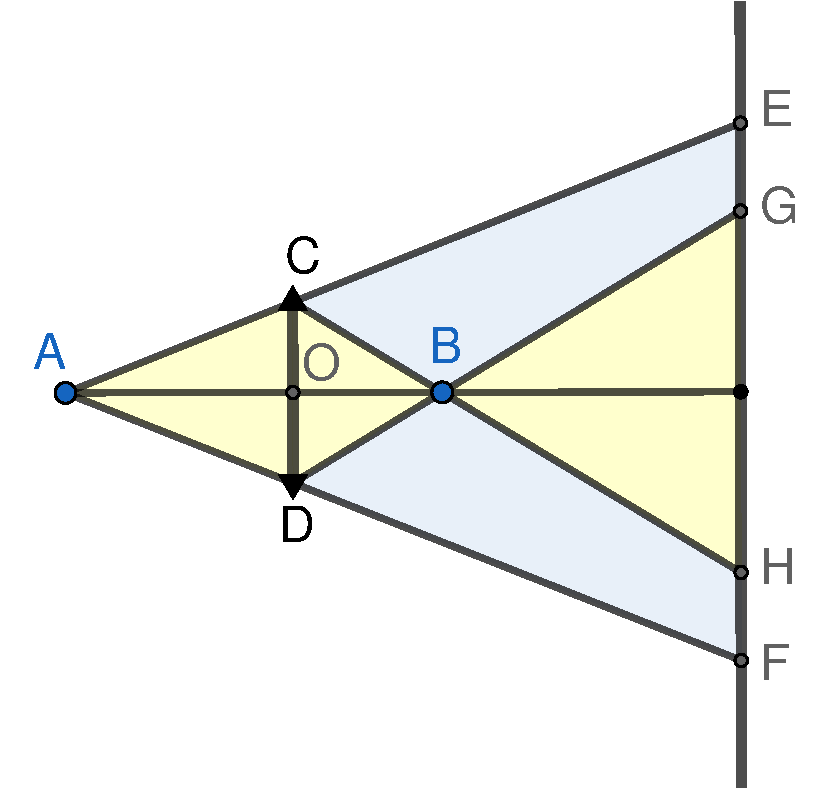
\includegraphics[width=\textwidth]{laatsekraan2}
  \end{minipage}
  \hfill
  \begin{minipage}[c]{0.60\textwidth}
    \vspace*{-2pt}
    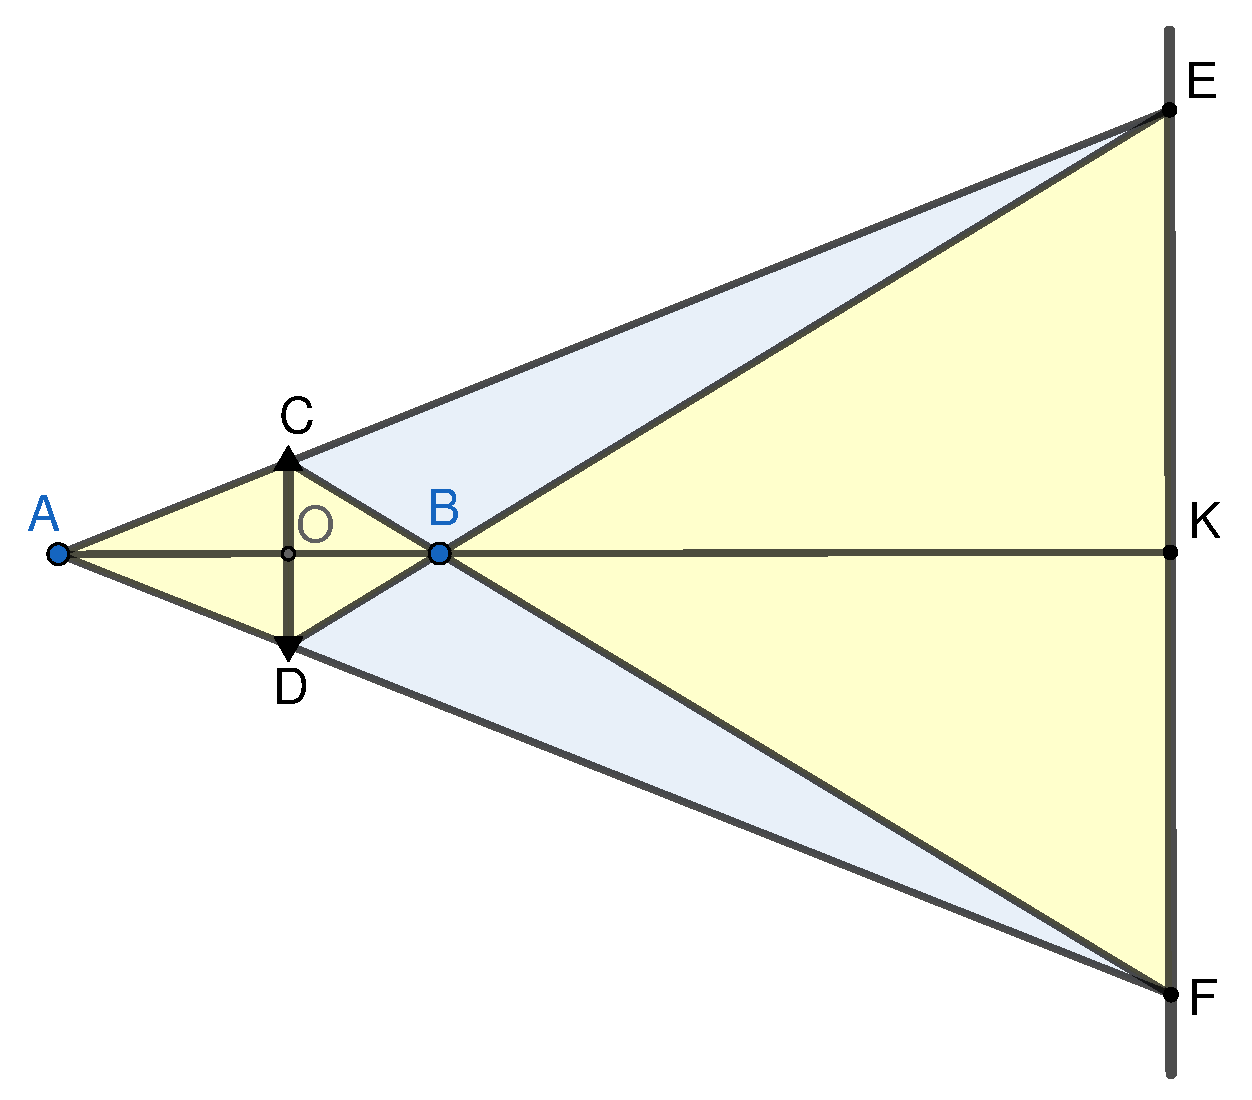
\includegraphics[width=\textwidth]{laatsekraan1}
  \end{minipage}
\end{figure}

Olgu $A$ valgusallikas, $B$ tema kujutis läätses ning $CD$ lääts.

Kui ekraan asub läätsest 10 ja 60 cm vahel, tekivad ekraanile kaks kontsentrilist ringi (vasakpoolne joonis): hele väiksem ring diameetriaga $GH$ asub tumeda ringi diameetriga $EF$ sees. Aladele EG ja HF valgusallika valgus ei jõua.

Eemdaldades läätse ekraanist saavad punktid $E$ ja $G$ kokku üheks nagu ka punktid $F$ ja $H$. Ekraani katab ühtlaselt valgus, nagu läätse poleks (parempoolne joonis).

Olgu $x=|AO|$ kaugus valgusallika ja läätse vahel, $r=|OC|$ läätse raadius ning $R=|KE|$. Ülesande tingimustest $|BO|=\SI{10}{cm}$, $|KO|=\SI{60}{cm}$ ning seega $|BK|=\SI{50}{cm}$. Sarnastest kolmnurkadest $AOC$ ja $AKE$ saame
\[
  \frac{r}{R}=\frac{x}{x+60}.
\]
Sarnastest kolmnurkadest $BOD$ ja $BKE$ aga
\[
  \frac{r}{R}=\frac{10}{50}.
\]
Kokkuvõttes saame võrrandi $\displaystyle{\frac{x}{x+60}=\frac{10}{50}}$, mille lahendiks on $x=\SI{15}{cm}$.

Läätse valemist nüüd
\[
  \frac{1}{10}+\frac{1}{15}=\frac{1}{f}\quad \Rightarrow \quad f=\SI{6}{cm}.
\]


\yl{SÕIT JÄÄL}
\punktid{8} \autor{Richard Luhtaru}
Kui auto mass on $m$, siis auto raskusjõud on $F_g = mg$ ja maksimaalne ratastele mõjuv hõõrdejõud on $F_h = \mu mg$. Maksimaalne autole mõjuda saav kiirendav/pidurdav jõud on maksimaalne hõõrdejõud (muidu hakkaksid rattad libisema), seega auto maksimaalne kiirendus on $a_{max} = \frac{F_h}{m} = \mu g$ ja minimaalne kiirendus on $a_{min}=-\frac{F_h}{m}= -\mu g$.

On ilmne, et minimaalse sõiduaja korral kiirendab auto kõigepealt maksimaalse kiirendusega $a_{max}$ ja seejärel pidurdab kiirendusega $a_{min}$, nii et auto jääks täpselt tee lõpus seisma. Tõepoolest, kui auto kiirendus ei oleks mingil hetkel maksimaalne/minimaalne võimalik, saaks auto sellel ajaperioodil lühikese aja maksimaalselt kiirendada ja pidurdada, vähendades sõiduaega. Kuna $\mu_2 > \mu_1$, siis on maksimaalne kiirendus suurem teisel lõigul ja seega ka kiirendamine muutub pidurdamiseks tee teisel lõigul.

Kulugu autol aeg $t_1$, et jõuda tee keskele, seejärel aeg $t_2$ jõudmaks kohta, kus kiirendamine muutub pidurdamiseks, ja seejärel aeg $t_3$, et jõuda tee lõppu. Vastavad auto kiirendused on $a_1=\mu_1 g$, $a_2=\mu_2 g$ ja $a_3=-\mu_2 g$.

Aja $t_1$ jooksul läbib auto teepikkuse $L$, seega
\[
  L=\frac{\mu_1 g t_1^2}{2} \implies t_1 = \sqrt{\frac{2L}{\mu_1 g}} = \SI{10}{s}.
\]
Tee keskele jõudes on auto kiirus
\[
  v_1 = \mu_1 g t_1 = \mu_1 g \cdot \sqrt{\frac{2L}{\mu_1 g}} = \sqrt{2L\mu_1 g} = \SI{10}{m/s}.
\]
Seejärel peale aja $t_2$ läbimist on auto kiirus
\[
  v_2 = v_1 + \mu_2 g t_2.
\]
Et teise lõigu pikkus on samuti $L$, siis
\[
  L = \frac{v_2^2 - v_1^2}{2a_2} + \frac{0-v_2^2}{2a_3} = \frac{2v_2^2 - v_1^2}{2\mu_2 g},
\]
\[
  v_2 = \sqrt{\frac{2\mu_2 gL+v_1^2}{2}} \approx \SI{12.25}{m/s}.
\]
Seega
\[
  t_2 = \frac{v_2-v_1}{\mu_2 g} \approx \SI{1.12}{s}.
\]
Kuna auto peab tee lõpus seisma jääma, siis
\[
  \Delta v = 0 \implies \mu_1 g t_1 + \mu_2 g t_2 - \mu_2 g t_3 = 0 \implies t_3 = t_2 + \frac{\mu_1}{\mu_2}t_1 \approx \SI{6.12}{s}
\]
ja tee läbimise koguaeg on
\[
  t=t_1+t_2+t_3 \approx \SI{17,24}{s}.
\]


\yl{VÕIMSUS}
\punktid{8} \autor{Kaur Aare Saar}
Vahetult pärast lüliti sulgemist käitub kondensaator kui lühis. Järelikult on skeemi kogutakistus
\[
  R=\frac{1}{\frac 1R + \frac 2{3R}}=\frac 35 R
\]
Pärast pika aja möödumist käitub kondensaator kui avatud lüliti. Seega takistus on
\[
  R=R+\frac{1}{\frac 1R + \frac 1{2R}}=\frac 53 R
\]
Võimsused on seega vastavalt $P=\frac{5V^2}{3R}$ ja $P=\frac{3V^2}{5R}$.


\yl{KEHA KERAL}
\punktid{10} \autor{Krister Kasemaa}
\osa Vaatleme keha liikumist ümber $\theta$ defineeritud ringjoone. Laiuskraadil $\theta$ avaldub väikese keha tiirlemisraadius kujul
\[
  r=R \: \cos \theta
\]
ja joonkiirus kujul
\[
  v= \omega r= \frac{2 \pi }{T} r = \frac{2 \pi R \: \cos \theta}{T}.
\]
Nüüd saab avaldada tsentrifugaaljõu:
\[
  F_{\mathrm{ kesk}}=\frac{m v^2}{r} =\frac{m \left(\frac{2 \pi R \: \cos \theta}{T}\right)^2}{R \: \cos \theta}=\frac{4 m \pi^2 R \: \cos \theta}{T^2}.
\]
Arvestades, et kaalule panustab ainult radiaalne tsentrifugaaljõu komponent
\[
  F_{\mathrm{\bot kesk}}= \cos \theta \; F_{\mathrm{ kesk}} = \frac{4 \pi^2 m R \: \cos ^2 \theta}{T^2},
\]
saab leida keha kaalu:
\[
  W=\frac{G m M}{R^2} - \frac{4 \pi^2 m R \: \cos ^2 \theta}{T^2} = m\bigg(\frac{G M T^2 - 4 \pi^2 R^3 \: \cos ^2 \theta }{R^2 T^2}\bigg).
\]
\osa Libisemist põhjustab tsentrifugaaljõu kera pinnaga tangentsiaalne komponent:
\[
  F_{\mathrm{kesk || }}= \sin(|\theta|) \; F_{\mathrm{ kesk}} = \frac{4 \pi^2 m R \: \cos \theta \sin(|\theta|)}{T^2}=\frac{2 \pi^2 m R \: \sin(|2\theta|)}{T^2} .
\]
Hõõrdeõud avaldub kujul
\[
  F_{\mathrm{h}}=\mu W = \mu \, m\left(\frac{G M T^2 - 4 \pi^2 R^3 \: \cos ^2 \theta }{R^2 T^2}\right).
\]
Seega, tasakaalu korral:
\[
  F_{\mathrm{kesk || }} \leq \mu W,
\]
\[
  \frac{2 \pi^2 m R \: \sin(|2\theta|)}{T^2} \leq
  \mu \, m\bigg(\frac{G M T^2 - 4 \pi^2 R^3 \: \cos ^2 \theta }{R^2 T^2}\bigg)
\]
ja järelikult
\[
  \mu \geq \frac{2 \pi^2 R^3 \: \sin(|2\theta|)}{G M T^2 - 4 \pi^2 R^3 \: \cos ^2 \theta }.
\]

\yl{KOLMNURK}
\punktid{10} \autor{Jaan Kalda}
Et osakesed liiguksid sirgjooneliselt, peaks see kolmnurk, mille tippudes need asuvad, jääma iseenesega sarnaseks. Et kolmnurga mediaanide lõikepunkt (massikese) jääb väliste jõudude puudumise tõttu paigale, siis peavad kõigile osakestele mõjuvad resultantjõud mõjuma piki mediaane ning nende moodulid peavad olema võrdelised vastavate mediaanide pikkustega (siis on mediaanide kasvamise kiiendused ja kiirused võrdelised mediaanide pikkustega ja kolmnurk jääb iseenesega sarnaseks).

Tähistame punktist $C$ lähtuvad küljed vektoritega $\vec a$ ja $\vec b$; tipust $C$ tõmmatud mediaan on $(\vec a+\vec b)/2$; sarnased avaldised saame ka ülejäänud mediaanide jaoks. Järelikult peavad osakestele mõjuvad resultantjõud avalduma kujul $p(\vec a+\vec b)=kq_C(\frac {\vec aq_B}{a^3}+\frac {\vec bq_A}{b^3})$, kus $p$ on konstant (sama kõigi osakeste jaoks kirjutatud avaldiste puhul) ning $k$ on Coulomb'i konstant. See võrdus kehtib ainult siis, kui $\frac {q_B}{a^3}=\frac {q_A}{b^3}$, st $q_Bb^3=q_Aa^3$. Analoogselt leiame, et  $q_Cc^3=q_Aa^3$, st $q_Aa^3=q_Bb^3=q_Cc^3\equiv Q$.

Kasutades siindefineeritud suurust  $Q$ saame avaldada konstandi $p=\frac {kQ}{a^3b^3c^3}$; sümmeetria tõttu on ilmne, et teiste osakeste jaoks saame täpselt samasuguse avaldise, nii nagu vajalik osakeste sirgjooneliseks liikumiseks. Seega: jah, iga kolmnurga puhul on võimalik osakeste sirgjooneline liikumine, vajalik on vaid rahuldada võrdus $q_Aa^3=q_Bb^3=q_Cc^3$.

\yl{VEESILINDER}
\punktid{12} \autor{Taavet Kalda}
\emph{Lahendus 1.} On selge, et kui veesammas ei kiireneks, oleks veesamba ülemise ja alumise punkti rõhkude vahe $\rho gh \approx 1.2p_0$ ning veesamba haripunktis oleks negatiivne rõhk. Aga kuna veesammas hakkab ühtse kehana teatud kiirendusega $a$ silindrist välja voolama (sest vesi on kokkusurumatu), siis liikudes veega kiirenevasse taustüsteemi, näeme et ülemise ja alumise punkti rõhkude vahe on tegelikult $\rho (g - a) h$ ning see ei pea tingimata negatiivne olema.

Vee välja voolamise käigus on peamine küsimus see, et mis vee asemel silindri üleval olevasse ruumi alles jääb. Üks variant on, et vee taha jääb vaakummull. Samas, kui vee rõhk langeb toatemperatuuril küllastunud veeauru rõhust madalamale, siis vee kontaktpinnas hakkab vesi aurustuma. Seega ei teki silindri ülemisse ossa mitte vaakum, vaid veeaurud rõhul $p_v$. Seega on veesamba ülemise ja alumise osa rõhkude vahe $p_0 - p_v = \rho (g - a)h$ ning veesammas kiireneb kiirendusega $a = g - (p_0 - p_v)/(\rho h) = \SI{1.62}{m/s^2}$.

\emph{Lahendus 2.} Vaatame veesambale mõjuvaid jõude. Olgu veesamba ristlõike pindala $S$. Siis alt mõjub õhurõhu poolt jõud $p_0 S$. Ülevalt sinna tekkiva küllastunud auru poolt jõud $p_v S$. Lisaks mõjub veesambale raskusjõud $mg$, kus veesamba mass on $m=\rho hS$. Newtoni II seaduse põhjal
\[
  ma=mg+p_vS-p_0S,
\]
kust leiame
\[
  a=g+\frac{(p_v-p_0)S}{m}=g+\frac{p_v-p_0}{\rho h}.
\]

\yl{VEDELIK PEEGLIL}
\punktid{12} \autor{Konstantin Dukatš}
\emph{Lahendus 1.} Kui meil on vedelik kõvera peegli peal, käitub see vedelik nagu lääts, mille ühe poole kõverusraadius on sama peegli kõverusraadiusega ja teise poole kõverusraadius läheneb lõpmatusele. Kuna peegli laius on palju väikse kui $l,h$, siis on tegemist õhukese läätsega. Sellisel juhul läätse optiline tugevus
\[
  D_l=\frac{1}{f_l}=\frac{n-1}{R},
\]
kus $n$ on vedeliku murdumisnäitaja ja $R$ on peegli kõverusraadius\footnote{Tegu on läätsevalmistaja valemi erikujuga. Läätsevalmistaja valem annab üldjuhul sfääriliste pindadega läätse tugevuse:
  \[
    D=\frac{1}{f}=(n-1)\left[\frac{1}{R_1}-\frac{1}{R_2}+\frac{(n-1)d}{nR_1R_2}\right],
  \]
  kus $f$ on läätse fookuskaugus, $n$ on läätse materjali murdumisnäitaja õhu suhtes, $R_1$ on valgusallikale lähema pinna kõverusraadius (koos märgikonventsiooniga), $R_2$ on valgusallikale kaugema pinna kõverusraadius ja $d$ on läätse paksus.
}. Peegli optiline tugevus
\[
  D_p=\frac{1}{f_p}=\frac{2}{R},
\]
kus $f_p$ on peegli fookuskaugus. Kuna valguskiired läbivad läätse kaks korda (enne peegeldamist ja pärast), siis läätse tugevusega peab arvestama kaks korda. Konbineerides läätse ja peegli saame, et
\[
  \frac{1}{a}+\frac{1}{k}=2 D_l+D_p,
\]
kus $a$ on objekti kaugus läätsest ja peeglist ning $k$ on kujutise kaugus läätsest ja peeglist. Avaldades $D_l$ ja $D_p$ saame, et
\[
  \frac{1}{a}+\frac{1}{k}=\frac{2(n-1)}{R}+\frac{2}{R}=\frac{2n}{R}
\]
Vee korral
\[
  \frac{1}{h}+\frac{1}{h}=\frac{2 n_v }{R} \implies R=h n_v.
\]
Tundmatu vedeliku korral
\[
  \frac{1}{h}+\frac{1}{h-l}=\frac{2 n_x }{R}.
\]
Avaldades $n_x$ saame, et
\[
  n_x =\frac{(2h-l)}{2h(h-l)} R =\frac{(2h-l)}{2(h-l)} n_v \approx \num{1.50}.
\]

\emph{Lahendus 2.}
Vaatleme allikast tulevat kiirt, mis on vertikaali suhtes nurga $\alpha$ all. Järelikult siseneb kiir vedelikku kaugusel $a = \alpha h$ peegli sümmetriateljest. Snelli seaduse kohaselt on kiire nurk vertikaali suhtest peale vedelikku sisenemist $\frac{\alpha }{n}$. Olgu kiire nurk peale peegli vastu peegeldumist $\beta$. Väikeste nurkade lähenduses on peegli pinna normaal nurga $\frac{1}{2} (\frac{\alpha}{n} + \beta)$ all. Samas lõikub peegli pinna normaal sümmeetriateljega kaugusel $R$, kus $R$ on nõguspeegli kõverusraadius. Seega,
\[
  \frac{1}{2} \left(\frac{\alpha}{n} + \beta\right) = \frac{a}{R} = \frac{\alpha h}{R},
\]
järelikult
\[
  \beta = \frac{2\alpha h}{R} - \frac{\alpha}{n}.
\]
Edasi, pärast peegeldumist ning vedelikust järjekordset väljumist on kiire nurk vertikaali suhtes
\[
  \gamma = \beta n = \frac{2\alpha nh}{R} - \alpha.
\]
Seega saame, et kujutise kaugus peegli pinnast on
\[
  \frac{1}{d} = \frac{\gamma}{a} = \frac{\gamma}{\alpha h} = \frac{2n}{R}- \frac{1}{h}.
\]
Kasutades saadud seost esialgses olukorras näeme, et
\[
  \frac{1}{h} = \frac{2n_v}{R} - \frac{1}{h}.
\]
Teisisõnu, $R = n_v h$. Pärast tundmatu vedelikuga asendamist saame aga
\[
  \frac{1}{h - l} = \frac{2n}{R} - \frac{1}{h} = \frac{2n}{n_v h} - \frac{1}{h}.
\]
Järelikult
\[
  n = \frac{2h-l}{h - l}\cdot  \frac{n_v}{2} \approx \num{1.5}.
\]

\yl{SIRGVOOL}
\punktid{14} \autor{Taavet Kalda}
Olgu sirgvool piki $z-$telge. Ampère'i seadusest näeme et sirgvool tekitab magnetvälja tugevusega $B_\varphi = \frac{\mu_0}{2\pi r}I$. Elektronile mõjub Lorentzi jõud $\vec F = -e\vec v \times \vec B$. Selleks et $v_z = \mathrm{const}$, peab elektroni radiaalne kiiruskomponent olema $0$. Tõepoolest, kui see ei oleks 0, siis kruvireegli järgi oleks Lorentzi jõul $z-$sihiline komponent ning seega $v_z$ ei saaks konstantne olla. Kuna magnetväli tööd ei tee, on elektroni kiirus konstantne ning seega $v_\varphi = \mathrm{const}$. Tegu on liikumisega pikki heeliksit raadiusega $r$.

Näeme et Lorentzi jõule panustab ainult $z$-sihiline kiiruskomponent ning et kruvireegli järgi on $F = ev_z B$ radiaalsuunaline. Lorentzi jõudu tasakaalustab kesktõmbekiirendus kujul
\[
-\frac{m_ev_\varphi^2}{r} = ev_z B = ev_z \frac{I \mu_0}{2\pi r}.
\]
Paneme tähele, et selle võrrandi lahendamiseks peab $v_z$ olema negatiivne. Asendades $v_\varphi^2 = v_0^2 - v_z^2$, saame
\[
m_e(v_z^2 - v_0^2) = ev_z \frac{I\mu_0}{2\pi}.
\]
Tegu on ruutvõrrandiga, lahendiks saame
\[
v_z = \frac{e I\mu_0}{4\pi m_e} \pm \sqrt{\left(\frac{e I\mu_0}{4\pi m_e}\right)^2+v_0^2}.
\]
Kuna $v_z < v_0$, on positiivne lahend ebafüüsikaline, st
\[
|v_z| = v_0 \left(\sqrt{\left(\frac{e I\mu_0}{4\pi m_e v_0^2}\right)^2 + 1} - \frac{e I\mu_0}{4\pi m_e v_0^2}\right).
\]

\end{document}
